\usetikzlibrary{arrows.meta,calc}
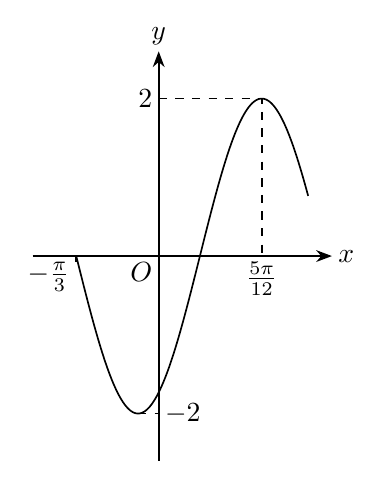
\begin{tikzpicture}[x=1cm,y=1cm,line width=.6pt,>=Stealth,font=\normalsize]
\draw[->] (-1.6,0)--(2.2,0) node[right,inner sep=0pt,xshift=2pt] {$x$};
\draw[->] (0,-2.6)--(0,2.6) node[above,inner sep=0pt,yshift=2pt] {$y$};
\node[below left,inner sep=0pt,xshift=-2pt,yshift=-2pt] at (0,0) {$O$};
\draw[dashed] (0,2)--(1.308,2)--(1.308,0);
\draw[dashed] (-0.2618,-2)--(0,-2);
\node[below,inner sep=0pt,yshift=-2pt,xshift=-10pt] at (-1.047,0) {$-\frac{\pi}{3}$};
\draw (-1.047,0)--(-1.047,-0.07);
\node[below,inner sep=0pt,yshift=-2pt] at (1.308,0) {$\frac{5\pi}{12}$};
\node[left,inner sep=0pt,xshift=-2pt] at (0,2) {$2$};
\node[right,inner sep=0pt,xshift=2pt] at (0,-2) {$-2$};
\draw[domain=-1.047:1.9,samples=200] plot (\x,{2*sin(deg(2*\x)-60)});
\end{tikzpicture}
